\documentclass[WHATMANUAL.tex]{subfiles}

\begin{document}

\chapter{Plotting the data}\label{chap:plotting_data}

WHAT make use of the powerful Python package Matplotlib to render the data in publication-quality graph with complex layout. With this tool and the way WHAT is built internally, there is almost no graph configuration that can't be done. The possibility are seldom limited by the UI and the time it requires to implement and design the addition of a new feature in the UI. It is however very fast to make changes in the source code to make your graph exactly the way it is desired. WHAT is buitl in a modular fashion. This means that it is not needed to run the entire program if only a certain feature is needed. For example, it is possible to plus the hydrograph from the Module Hydroprint of WHAT without the UI. If you have any idea, suggestion or request, please contact us. We would like to hear from you. For example, changing the color, adding a legend or plotting multiple water level time series on a same graph is something that can be easily achieved by modifying the source code, but that can take a lot of time to implement in a good and robust UI design.

The tradeoff for the packaging of code into a UI is that the production of graph in the frame of WHAT UI is more strict and allow for less flexibility to the user. Neverthless, it is still possible to produce very good graph from the UI and new options are added frequently to the program to add more flexibility.

The plotting of the weather and water-level data into a same graph in a publication-quality figure is done in the mode ``Layout'' in the tab called ``Hydrograph'' (see Figure~X).

\begin{figure}[h!]
\centering
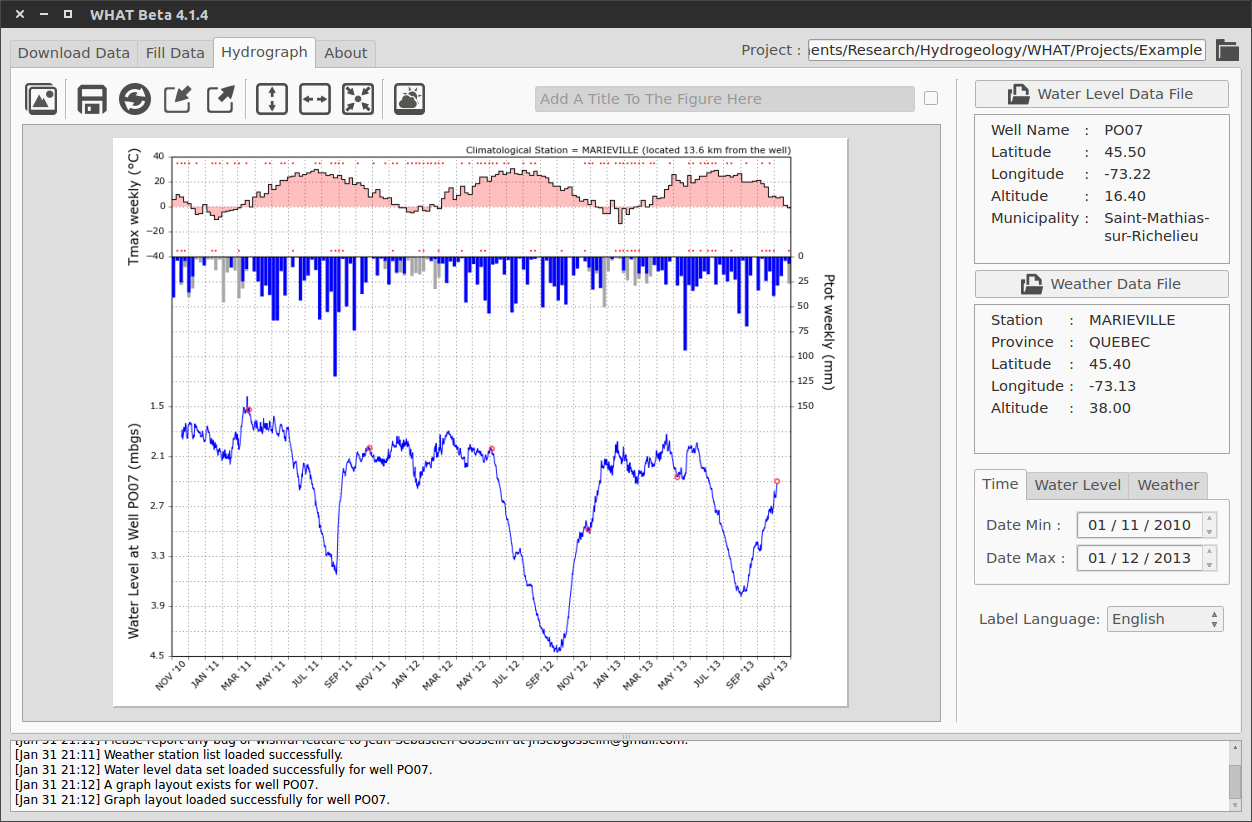
\includegraphics[width=0.75\textwidth]{img/WHAT_Screenshot002}
\caption[Mode ``Layout'' of the Tab ``Hydrograph'']{Mode ``Layout'' of the Tab ``Hydrograph''.}
\label{fig:tab_hydrograph_layout}
\end{figure}

The mode Layout and Computation both shares the same data. This means that when importing a water level data file or a weather data file in one mode, will affect the content of the other. Thus, the process of importing water level data is the same as the one explained previously in section X. When a water level data file is loaded into memory, the weather data file of the station closest to the well will also be loaded if the folder Output is not empty and will produce a graph with both of these data series. If a weather data file is loaded before a water level data file, only the weather data series will be plotted. It is possible to disable the plotting of either the weather data file or the water-level time series at anytime in order to plot one or the other dataset alone in a single graph. The purpose of this mode is not to explore interactively the data, nor to conduct computation, but to produce publication-quality graph from the data.

The tab hydrograph is equiped of a toolbar at the top and a right panel that is used to edit the graph. By design, it is not possible to interactively modify the content of the graph that is being produced. WHAT display the figure in a bitmap format for performance purposes. The figure however when saved in a pdf or svg format will be fully vectorial for publication-quality work. The figure can be panned by draggin the mouse with the mouse button depressed. Zoom in by pressing the Ctrl key while moving the mouse wheel up and zoom out with mouse wheel down.

\section{Hydrograph Overview}

The main feature of this tab is the production of a publication=quality figure that contains both the water-level and weather time-series.

\section{Toolbar}

The toolbar offers various tool that are mostly composed of single action button for automatic formating of the data in the figure. From left to right:\vspace{0.5cm}

%http://tex.stackexchange.com/questions/85208/vertically-align-cell-table-in-figure
%http://tex.stackexchange.com/questions/16258/how-can-the-margins-around-a-table-set-to-0pt
\noindent
\begin{tabular}{@{}p{0.085\textwidth}@{}@{}p{0.915\textwidth}@{}}
\adjustbox{valign=t}{
\includegraphics[width=1cm]{img/toggleMode2}} & The toggle button is used to switch from one mode to the other. As said previously, both mode shares the same data. Hence, doing manipulation on the dataset in "Edit" mode will impact what is plotted in the "Layout" mode. Alternatively, loading a new water level data file will impact both the Edit and Layout mode at the same time. It is possible to switch from one mode to the other at anytime without losing the work that is in progress. Hence, both mode can be used concurrently to edit and analyse the data.
\end{tabular}\vspace{0.5cm}

\noindent
\begin{tabular}{@{}p{0.085\textwidth}@{}@{}p{0.915\textwidth}@{}}
\adjustbox{valign=t}{
\includegraphics[width=1cm]{img/save}} & Allow to save the current hydrograph figure either in pdf or svg format. In both format the image is saved in a vectorial format. To convert the figure in a bitmap format such as png, jpg or tiff, software such as acrobat adobe or the very good open source software GIMP can be used. Inkscape is also a very good open source vectorial image editing software that can both work in pdf or svg format.
\end{tabular}\vspace{0.5cm}

\noindent
\begin{tabular}{@{}p{0.085\textwidth}@{}@{}p{0.915\textwidth}@{}}
\adjustbox{valign=t}{
\includegraphics[width=1cm]{img/refresh2}} & This button is used mainly for debugging purpose and for experimental features that are not fully integrated in the UI yet. It forces a complete redrawing of the hydrograph.
\end{tabular}\vspace{0.5cm}

\noindent
\begin{tabular}{@{}p{0.085\textwidth}@{}@{}p{0.915\textwidth}@{}}
\adjustbox{valign=t}{
\includegraphics[width=1cm]{img/save_config}} & This button is used to save the current graph layout for future uses. The layout is saved in the file ``graph\_layout.lst'' located in the project folder and is referenced with the ID of the well.
\end{tabular}\vspace{0.5cm}

\noindent
\begin{tabular}{@{}p{0.085\textwidth}@{}@{}p{0.915\textwidth}@{}}
\adjustbox{valign=t}{
\includegraphics[width=1cm]{img/load_config}} & This button is used to force the loading of a previously saved layout associated with the current well. When loading a water-level data file in memory, WHAT will automatically check if there is a layout already saved for that well and will ask the user if he wants or not to load it. If the user refuses, WHAT will try to to a best fit of the data automatically to produce the figure.
\end{tabular}\vspace{0.5cm}

\noindent
\begin{tabular}{@{}p{0.085\textwidth}@{}@{}p{0.915\textwidth}@{}}
\adjustbox{valign=t}{
\includegraphics[width=1cm]{img/search_closest_weather_station}} & The Best Fit buttons are used to force a refitting of the water level data in the vertical axis and in the time axis respectively. This tool does not presently work very well if there is aberrant data in the time-series or if the is a long recuperation curve at the beginning of the dataset following the boring of the well.
\end{tabular}\vspace{0.5cm}

\noindent
\begin{tabular}{@{}p{0.085\textwidth}@{}@{}p{0.915\textwidth}@{}}
\adjustbox{valign=t}{
\includegraphics[width=1cm]{img/search_closest_weather_station}} & This function is used to force WHAT to search for the weather data file in the folder Output of the weather station that is closest to the well, to load it in memory and to plot the results in the hydrograph figure.
\end{tabular}\vspace{0.5cm}

\section{Right Panel}

The water level and weather data file section of the Right panel are shared by both mode of the tab hydrograph. 

\section{Water Level Datum}

If an appropriate value of the altitude of ground surface at the well location is provided in the header of the input file, it will be possible to switch the datum of the water level when plotting the data from Meters Below Ground Surface (mbgs) to Meters Above Sea Level (masl).

In computation mode however, data are always displayed as meter above ground surface, with the values positive when above ground surface and negative when below. Displaying water-level time-series relative to the ground surface is much more useful than relative to mean sea level or as the height of the water column above the instrument.By displaying the value relative to the ground surface, it is easy to see the width of the unsaturated zone water has to pass through to attained the water table and become groundwater recharge. Depth of the unsaturated zone is a major factor in the delai between the response of the water table to precipitation or snowmelt event and it also play a role in the attenuation of the signal. Moreover, knowing the depth of the water level below the ground surface also gives indication about possible evapotranspiration from the water-table and also flood event.

In Layout mode it is possible to plot the water level relative to four different datum:

- meters above ground surface (mags)
- meters below ground surface (mbgs)
- meters above logger (mal)
- meters above see level (masl)

mags and mbgs options have the same reference point, but the vertical axis is inverted in the case of mbgs, with the water level being positive below the ground surface and increasing in value as the depth to the surface increase.

\end{document}